\section{Топологический изолятор на основе \\квантовой ямы HgTe}
\subsection{Эффективный гамильтониан}
Хотя впервые предложенный топологический изолятор --- графен \cite{Kane2005}, 
первая экспериментальная реализация топологического изолятора ---
квантовая яма CdTe--HgTe--CdTe. Она представляет собой узкий (несколько нанометров)
двумерный слой HgTe, заключённый между CdTe. Как CdTe, так и HgTe --- вещества 
с сильным спин--орбитальным взаимодействием, которое приводит к расщеплению p--зоны.
Образуются зоны лёгких и тяжёлых дырок, которые вместе преобразуются как спин $3/2$,  
и отщеплённая зона со спином $1/2$, которая лежит ниже по энергии. Отличие CdTe и HgTe ---
в положении $s$--зоны. В CdTe она является зоной проводимости и лежит выше лёгких и тяжёлых
дырок. Поэтому CdTe --- полупроводник. HgTe обладает инвертированной зонной структурой:
s--зона лежит ниже тяжёлых и лёгких дырок. Из--за этого HgTe -- полуметалл. 

В квантовой яме вместо трёхмерного спектра HgTe возникают двумерные 
уровни размерного квавнтования, которые можно найти, используя гамильтониан Кейна 
\cite{Kane1957}. Это 
было впервые сделано в \cite{Bernevig2006}. Мы повторили их вычисления, они приведены в 
приложении~\ref{app:dim_quant}.
При малой толщине ямы <<доминирует>> спектр CdTe, поэтому 
зонная структура ямы нормальная: E1--подуровень размерного квантования выше HH1 подуровня. 
Однако в некоторый момент происходит их пересечение, после чего они меняются местами. Когда 
уровни размерного квантования близки друг к другу, их можно описывать с помощью эффективного
$k\cdot p$ гамильтониана. Оказывается, что этот эффективный гамильтониан описывает
топологический изолятор.

\begin{figure}[h]
    \centering
    \begin{minipage}[t]{0.45\textwidth}
        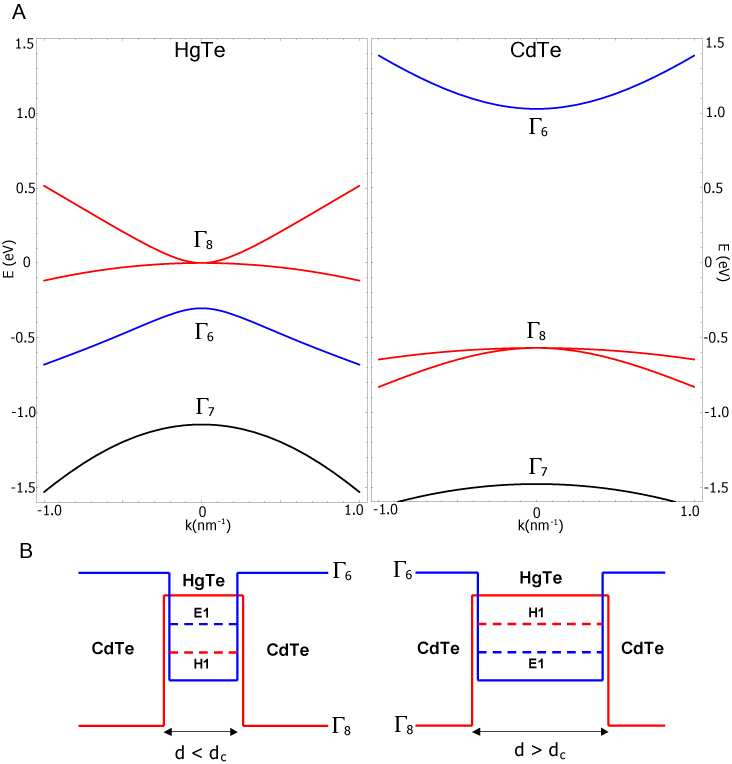
\includegraphics[width=0.9\linewidth]{quantum_well.png}
        \caption{Объемный спектр HgTe и CdTe и 
                 схематическое изображение квантовой ямы}
    \end{minipage}
    \hfill
    \begin{minipage}[t]{0.45\textwidth}
        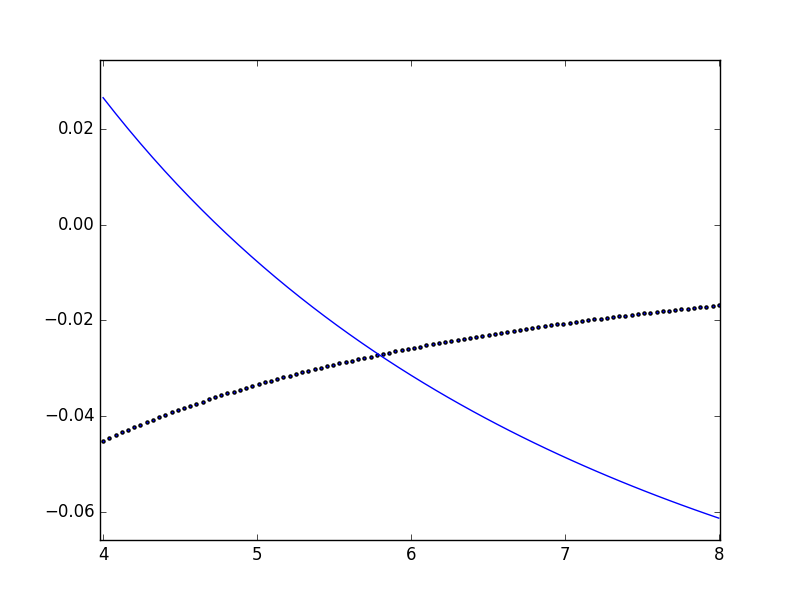
\includegraphics[width=0.9\linewidth]{levels.png}
        \caption{Уровни размерного квантования}
    \end{minipage}
\end{figure}

Эффективный гамильтониан (с учётом спинов) принимает вид
\begin{equation}
    H = \begin{pmatrix}
            \xi + \frac{p^2}{2m_1} & v(p_x - ip_y) & 0 & 0 \\
            v(p_x + ip_y) & -\xi - \frac{p^2}{2m_2}& 0 & 0 \\
            0 & 0 & \xi + \frac{p^2}{2m_1} & v(p_x + ip_y) \\
            0 &  0 &  v(p_x - ip_y) & -\xi - \frac{p^2}{2m_2}
        \end{pmatrix}
\end{equation}
